\begin{chapter}{Implementacja głównej aplikacji WikiGraph}
	\newcommand{\chapterPath}{rozdzialy/4_implementacja}

	W tym rozdziale opisana zostanie implementacja aplikacji wizualizującej graf połączeń. Zostanie omówiony przyjęty model danych oraz sposób ich wczytywania. Następnie rozwinięta zostanie kwestia reprezentacji węzłów i połączeń oraz integracji aplikacji ze środowiskiem jaskini. Na koniec zostaną zestawione opisy pozostałych elementów interfejsu i funkcjonalności. 
	
	\section{Model danych}
\sectionauthor{Stanisław Góra}

Model danych aplikacji tworzony jest na podstawie plików opisanych w sekcji \ref{sec:data-files}. Są one otwierane jako strumienie używając klasy \codeinline{FileStream} co pozwala na jednakowy dostęp do każdej części pliku. 

Listing \ref{lst:node-model} zawiera używany przez aplikację model węzła. Przy żądaniu załadowania do pamięci węzła o konkretnym numerze (\ref{line:nm-id}) najpierw odczytywane są informacje z pliku mapy a następnie na ich podstawie wczytywany jest tytuł (\ref{line:nm-title}) oraz połączenia węzła (\ref{line:nm-children} i \ref{line:nm-parents}). Określany jest też typ węzła (\ref{line:nm-type}) oraz jego identyfikator przypisany przez Wikipedię (\ref{line:nm-wikiid}). Na koniec nowo wczytanemu węzłowi zostaje przypisany stan (\ref{line:nm-state}) aktywny.
\begin{lstlisting}[caption={Model węzła grafu}, label=lst:node-model]
public class Node {
	public uint[] Children; %*\label{line:nm-children}*)
	public uint[] Parents; %*\label{line:nm-parents}*)

	public readonly uint ID; %*\label{line:nm-id}*)
	public uint WikiID; %*\label{line:nm-wikiid}*)

	public string Title; %*\label{line:nm-title}*)

	public NodeType Type; %*\label{line:nm-type}*)
	public NodeState State; %*\label{line:nm-state}*)
	%*\dots*)
}
\end{lstlisting}

Załadowane węzły są dodawane jako wartości w mapie ID $\,\to\,$ \codeinline{Node} co pozwala na późniejsze szybkie uzyskanie modelu na podstawie jego identyfikatora. Przechowywanie grafu w pamięci zostanie szczegółowo opisane w sekcji \ref{sec:graf-reprezentacja}.

W wyniku interakcji użytkownika z węzłem pokazywane są połączenia, Zostały one zamodelowane jako zbiór dwóch węzłów. Przy tym przyjmujemy że połączenie zaczyna się w węźle z którym nastąpiła interakcja.

	\section{Wizualna reprezentacja węzłów i połączeń}
\label{sec:graf-reprezentacja}
\newcommand\mapitem[3]{
	\item \textbf{#1 $\,\to\,$ #2}

	#3
}

% Przechowywanie grafu w pamięci
\noindent
Graf jest przechowywany w pamięci aplikacji jako zbiór map:
\begin{enumerate}[label=\textbullet]
	\mapitem{Identyfikator węzła}{Model węzła}{Opisana już mapa warstwy modelu}
	\mapitem{Model węzła}{Obiekt wizualny węzła}{Przechowuje widoczne aktualnie w aplikacji węzły jako wartości przypisane do modelu reprezentowanego węzła. Obiekt wizualny przechowuje numer ID węzła co zamyka pętlę powiązań i w efekcie pozwala na uzyskanie informacji o węźle (z jego modelu) mając na wejściu jego obiekt wizualny na podstawie dwóch map.}
	\mapitem{Model połączenia}{Obiekt wizualny połączenia}{Mapa analogiczna do poprzedniej, przechowująca informacje o połączeniach między węzłami. Podobnie obiekt wizualny połączenia przechowuje dwa identyfikatory węzłów które łączy.}
	
	\mapitem{Model połączenia}{Obiekt wizualny reprezentacji węzła końcowego połączenia}{Mapa przechowująca pomocnicze reprezentacje węzłów końcowych połączenia opisane szczegółowo w \ref{sec:tryby-widoki}.}
\end{enumerate}

% GO Node - Billboard Shader
\paragraph{Reprezentacja węzła} Z uwagi na dużą ilość jednocześnie załadowanych węzłów (kilka do kilkunastu tysięcy na raz) konieczne okazały się pewne optymalizacje poprawiające szybkość działania aplikacji. 

Obiekty węzłów nie są w większości przypadków tworzone dynamicznie. Zamiast tego przy starcie aplikacji tworzona jest pula nieużywanych obiektów. W momencie ładowania węzła nowy obiekt wizualny tworzony jest tylko w przypadku kiedy pula została wyczerpana. Przy usuwaniu węzła jego reprezentacja nie jest niszczona tylko zwracana do puli w celu przyszłego wykorzystania.

W celu odciążenia karty graficznej zrezygnowaliśmy z wyświetlania każdego węzła jako trójwymiarowego modelu (jak na przykład kuli). Reprezentacją węzła jest prosta grafika rastrowa. Jest ona dużo szybsza do przetworzenia ponieważ zawiera tylko cztery wierzchołki - jest to kwadratowa płaszczyzna z nałożoną teksturą. Dzięki temu jesteśmy w stanie wyświetlić więcej węzłów na raz bez utraty płynności działania aplikacji.

Takie rozwiązanie powoduje jednak pewną komplikację. Płaszczyzna z grafiką, w przeciwieństwie do przestrzennego modelu, jest dobrze widoczna tylko kiedy kamera jest ustawiona bezpośrednio przed nią. Pojawia się więc potrzeba obracania obiektu węzła tak aby był on zawsze zwrócony przodem do użytkownika zwiedzającego graf. Najprostszym rozwiązaniem byłoby dodanie krótkiego skryptu do każdego obiektu który przy każdym odświeżeniu ekranu obracałby reprezentację węzła w stronę kamery. Nie jest to jednak dobre rozwiązanie z powodu narzutu czasowego. W każdej klatce ta sama operacja byłaby wykonywana potencjalnie kilkanaście tysięcy razy co mogłoby mieć widoczny efekt na szybkości działania.

Poprawnym rozwiązaniem jest użycie shadera. W przeciwieństwie do standardowych skryptów aplikacji jego działanie jest zrównoleglone przez kartę graficzną dla potencjalnie każdego przetwarzanego wierzchołka. Tu jednak natrafiliśmy na kolejny problem. Powszechnie stosowane są tak zwane ``Billboard Shadery'' które służą dokładnie do interesującego nas celu, jednak w szczególnym przypadku aplikacji budowanej na środowisko LZWP są niewystarczające. Każda ściana jaskini jest kontrolowana przez osobny komputer z osobną instancją aplikacji posiadającą osobną kamerę skierowaną w kierunku danej ściany. Billboard Shader odwraca obiekty węzłów w kierunku kamery na lokalnej ścianie co powoduje że jeśli dany obiekt znajdzie się w pozycji wyświetlanej na przecięciu ekranów (połowa węzła na jednej a połowa na drugiej ścianie jaskini), na każdym z odpowiadających za ściany komputerów zostanie obrócony w lekko innym kierunku. W efekcie części obiektu węzła mogą nie być spójne.

Aby rozwiązać ten problem należało wybrać obiekt wspólny dla wszystkich ścian a następnie obracać grafiki węzłów w stosunku do niego zamiast do kamer. To wymagało ręcznego przepisania shadera ponieważ nie jest częstym problemem którego rozwiązanie byłoby ogólnie dostępne do użycia.

% GO Connection - B-Spline
\paragraph{Reprezentacja połączenia} 


	\section{Tryby poruszania się i widoki węzła}

	\section{Elementy zwiększające użyteczność aplikacji}
\sectionauthor{Mikołaj Mirko}
\label{sec:elementy}
Jednym z ważniejszych elementów znajdujących się w aplikacji jest podążający za wzrokiem nagłówek z informacjami o stanie grafu. Umiejscowiony jest on powyżej linii wzroku tak, aby nie przeszkadzał w interakcji z węzłami, a zarazem był wyraźnie widoczny z każdego miejsca oraz kąta patrzenia. Jego pozycja pionowa jest zaczepiona w stałym punkcie, a pozycja pozioma uzależniona od kierunku wyznaczanego przez główne okulary jaskini.

Na samej górze znajduje się informacja o tym, czy węzeł jest tylko wskazywany kontrolerem, czy jesteśmy w widoku grafu z aktualnie wybranym węzłem. Zaraz pod spodem widoczny jest tytuł artykułu lub kategorii. W trybie swobodnego latania nagłówek wyświetlany jest tylko w przypadku wskazywania węzłów. Rysunek \ref{fig:header1} nakreśla układ nagłówka po wskazaniu artykułu ``Matematyka''. Jeśli węzeł posiada jakieś połączenia, ich liczba wyświetlana jest pod tytułem.

\img{\chapterPath/img/header1.png}{Nagłówek po wskazaniu węzła}{header1}{.8}

Dla widoku węzła dostępna jest większa ilość informacji. Pod tytułem pojawia się podłużny wskaźnik przypominający poziomy pasek przewijania. Wraz z informacją tekstową, znajdującą się tuż pod nim, określa aktualnie wyświetlany wycinek listy połączeń. Łatwo zauważyć, które połączenia są wyświetlane wokół użytkownika oraz jaką część stanowią. Na Rysunku \ref{fig:header2} wybrany został artykuł zatytułowany ``Wstęga Möbiusa'' z 21 połączeniami wychodzącymi (aktualnie wyświetlane są połączenia od pierwszego do ósmego włącznie).

\img{\chapterPath/img/header2.png}{Nagłówek w widoku węzła z informacją o połączeniach}{header2}{.8}

Ostatnią częścią nagłówka jest ikona stanu. Zawiera ona 3 istotne informacje: rodzaj węzła (artykuł lub kategoria), aktualny typ połączeń (wychodzące z węzła lub do niego trafiające) oraz wariant poruszania się. Rodzaj węzła jest ilustrowany poprzez kolor oraz kształt (Rysunek \ref{fig:node_sprites}). O typie połączeń świadczy również kolor, a także skierowanie strzałek w stosunku do symbolu węzła. (Na Rysunku \ref{fig:header2} ikona oznacza artykuł z połączeniami wychodzącymi). Domyślnym wariantem poruszania się jest ręczne przeskakiwanie z węzła na węzeł. Przy uruchomionej zaprogramowanej trasie (czyli automatycznym przechodzeniu po zdefiniowanej ścieżce - więcej o tym w sekcji \ref{sec:history}) na symbolu węzła pojawia się fraza \textit{AUTO} (Rysunek \ref{fig:header3}).

\img{\chapterPath/img/header3.png}{Nagłówek z ikoną stanu sygnalizującą trwające automatyczne przemierzanie trasy}{header3}{.8}

Aplikacja została dodatkowo wyposażona w elementy wspomagające pracę z grafem. Na dolnym ekranie widoczne są półprzezroczyste linie pomocnicze określające płaszczyznę podłoża. Przemieszczają się one z kamerą i mają na celu zapewnienie punktu odniesienia do innych obiektów otaczających użytkownika. Opisana siatka widoczna jest na Rysunku \ref{fig:widok_wezla}.

Kolejnym elementem jest przestrzeń pomocy. Jest to specjalna przestrzeń wydzielona od struktury grafu, do której można wejść w dowolnej chwili korzystania z aplikacji. Użytkownik jest w niej umieszczany również na starcie programu. Zawiera ona podstawowe informacje o programie, a także zestaw infografik zapoznających użytkownika ze sposobami sterowania i możliwościami aplikacji (Rysunek \ref{fig:info_space}).

\img{\chapterPath/img/info_space.png}{Jedna z infografik dostępnych w przestrzeni pomocy}{info_space}{.8}

Dodatkowo do aplikacji została dodana specjalnie stworzona do tego celu muzyka. Przez cały czas działania aplikacji w tle odtwarzany jest klimatyczny ambient wzmacniający immersję. Ponadto każda akcja użytkownika ma przypisany inny efekt dźwiękowy. Sygnalizuje ona użytkownikowi, że aplikacja poprawnie odebrała wciśnięcie przycisku, co zwiększa intuicyjność sterowania. Ponadto sygnalizuje specjalne akcje takie jak zmiana trybu przeglądania, czy włączenie lub wyłączenie pomocy.
	\section{Historia przegl�dania oraz zaprogramowane trasy}
Specyfika dzia�ania aplikacji, zwi�zana z wykonywaniem przez u�ytkownika akcji nawigacyjnych, oraz �rodowisko dzia�ania sk�oni�y do zaimplementowania funkcjonalno�ci zwi�zanych z histori�. Znacz�co u�atwi� i przyspiesz� one poruszanie si� po w�z�ach grafu. Bez mo�liwo�ci skorzystania z historii u�ytkownik by�by zmuszony do ka�dorazowego szukania poprzedniego w�z�a  w grafie b�d� w odpowiednim widoku wybranego w�z�a. Co wi�cej, aby zapewni� powtarzalno�� podczas prezentacji, a tak�e, aby wyeksponowa� ciekawe przypadki po��cze� pomi�dzy w�z�ami, b�dzie mo�liwe zapisanie tras przegl�dania. Odtwarzanie tras umo�liwia dok�adne planowanie prezentacji i eliminuje problemy wynikaj�ce z losowo�ci wy�wietlania w�z��w. 

Do historii zapisywane s� tylko akcje kluczowe dla nawigacji - zmiana widoku wy�wietlania oraz wybieranie w�z��w. Inne dzia�ania u�ytkownika nie powoduj� znacz�cych zmian w nawigacji po grafie i ich przechowywanie jest bezcelowe. Po naci�ni�ciu Przycisku 2 na kontrolerze wywo�ywana jest poprzednia akcja wykonana przez u�ytkownika. Odpowiednio, aby ponowi� cofni�t� akcj�, nale�y nacisn�� Przycisk 3. W przypadku braku akcji do ponowienia lub cofni�cia nie jest podejmowane �adne dzia�anie. Wywo�ywanie i zapisywanie tras dost�pne jest z poziomu konsoli operatora opisanej w nast�pnym punkcie.


Akcje u�ytkownika s� przechowywane jako odpowiednie klasy dziedzicz�ce po klasie UserAction. Posiada ona wirtualne funkcje Execute() oraz UnExecute() s�u��ce odpowiednio ponawianiu i cofaniu akcji. Ka�da akcja posiada tak�e swojego w�asnego delegata, zale�nego od typu akcji. 

Bezpo�rednie operacje na historii wykonywane s� przez HistoryService. Przechowuje on akcje u�ytkownika we dwu stosach: pierwszy s�u�y zapisywaniu akcji do cofni�cia, drugi akcji do ponowienia. W momencie wci�ni�cia przycisku 2 wyzwalane jest zdarzenie wywo�uj�ce funkcj� UndoAction(), kt�ra poza wykonaniem kolejnego zdarzenia wywo�uj�cego funkcj� akcji odpowiedzialnej za cofanie, zdejmuje t� akcj� ze stosu akcji do cofania i wk�ada na stos akcji do ponawiania.

Wszystkie delegowane funkcje s�u��ce historii oraz trasom s� przypisywane w kontrolerze HistoryController. Warunkiem jest, aby aplikacja by�a serwerem.

Zaznaczanie w�z��w z historii oraz zmiana widoku odbywa si� w identyczny spos�b, jak zwyk�e wywo�ywanie tych akcji przy u�yciu kontrolera, jednak nie s� one ponowne zapisywane do historii, jak przy zwyk�ym wywo�aniu.

Analogicznie do modu�u historii zaprojektowane zosta�o odtwarzanie tras. Pliki zawieraj�ce trasy posiadaj� rozszerzenie .wgroute. Struktura pliku jest stosunkowo prosta - pierwsza cyfra s�u�y rozr�nieniu akcji u�ytkownika: 0 oznacza zmian� widoku, a 1 wybranie w�z�a. W przypadku zmiany widoku po �redniku mo�na znale�� cyfr� 0 lub 1. 0 odpowiada zmianie widoku na na widok dzieci, a 1 zmianie widoku na widok rodzic�w. Je�li akcj� by�o wybranie w�z�a, po �redniku znajduje si� ID artyku�u do wybrania. 

Po wybraniu trasy rozpoczyna si� proces jej wczytywania. S� za to odpowiedzialne dwie klasy: RoutesReader oraz RoutesLoader. Pierwsza ma za zadanie pobra� dost�pne trasy, ich nazwy i d�ugo�� oraz wczytywa� kolejne linijki plik�w. Druga przekszta�ca wczytane dane linijka po linijce na odpowiednie akcje i dopisuje do stosu.

W momencie w��czenia trasy inicjowane jest wczytanie trasy z plik�w, a po tej operacji tworzony jest wsp�program(ang. coroutine), kt�ra ma za zadanie wykonywanie kolejnych akcji trasy co dan� liczb� sekund. Odtwarzanie trasy sygnalizowane jest przez ikon� AUTO w nag��wku. W ka�dym momencie mo�liwe jest wy��czenie odtwarzania trasy za pomoc� Przycisku 4, powoduj�cego zatrzymanie wsp�programu. W przypadku w��czenia innej trasy w trakcie odtwarzania, wsp�program poprzedniej trasy jest tak�e wy��czany, a nast�pnie wczytywana i inicjalizowana jest nowa trasa. 


	\section{Integracja z jaskinią rzeczywistości wirtualnej}
\sectionauthor{Stanisław Góra}
Laboratorium Zanurzonej Wizualizacji Przestrzennej \cite{LZWP_article} posiada szereg innowacyjnych rozwiązań z zakresu rzeczywistości wirtualnej. Największą instalacją jest wykorzystywana w tym projekcie duża jaskinia będąca sześciennym pomieszczeniem o boku 3,4m. Na każdą ze ścian wyświetlany jest z zewnątrz obraz z dwóch projektorów zdolnych stworzyć projekcję stereoskopową odbieraną przy pomocy okularów migawkowych \cite{IntegraAV}. Sterowanie symulacją odbywa się poprzez użycie kontrolera z joystickiem oraz pięcioma przyciskami. Dodatkowo zainstalowany jest system śledzenia ruchu pozwalający na wykrycie położenia kontrolera oraz okularów osoby sterującej symulacją.

% LZWPLib
Przystosowanie aplikacji do działania w środowisku LZWP dzieli się na dwa podzadania: obsługa wejścia użytkownika oraz synchronizacja stanu aplikacji pomiędzy komputerami obsługującymi ściany jaskini. Reszta integracji jest zapewniana przez stworzoną przez pracowników LZWP bibliotekę.

% Input Module
\subsection{Moduł wejścia}
W założeniu aplikacja ma wspierać dwie metody interakcji użytkownika, nazywane później środowiskami:
\begin{enumerate}[label=\textbullet]
	\item \textbf{PC} - gdzie użytkownik posługuje się klawiaturą i myszą, używane głównie podczas procesu wytwarzania aplikacji
	\item \textbf{Jaskini} - gdzie użytkownik nosi okulary i trzyma specjalny kontroler nazywany flystickiem
\end{enumerate}
Aby ułatwić sobie wytwarzanie głównej logiki aplikacji, wejście zostało odseparowane w osobny moduł, który może być przed uruchomieniem ustawiony w jeden z dwóch trybów, odpowiadającym każdemu środowisku. Tryb ten definiuje jakiego rodzaju wejścia ma nasłuchiwać aplikacja. Moduł wejścia składa się z trzech mniejszych części:
\paragraph{Definicje akcji użytkownika}
Ustala wspólny interfejs dla każdej akcji użytkownika dostępnej w aplikacji. Są to między innymi: 
\begin{enumerate}[label=\textbullet]
	\item Użycie przycisku klawiatury i myszy (PC) lub flysticka (jaskinia)
	\item Przesunięcie myszy (PC) lub flysticka (jaskinia)
\end{enumerate}
Oprócz tego jest odpowiedzialna za nasłuchiwanie wykonania przez użytkownika swojej akcji i odpowiednie powiadomienie aplikacji.

\paragraph{Definicje akcji aplikacji}
Spis akcji wykonywanych w aplikacji. Są to między innymi: 
\begin{enumerate}[label=\textbullet]
	\item Wybranie lub podświetlenie węzła
	\item Poruszanie się po grafie
	\item Zmiana zakresu wyświetlanych połączeń
\end{enumerate}
Każda akcja ma swój typ (opisany w poprzednim punkcie). Dostępny jest też interfejs, dzięki któremu możliwe jest łatwe wybranie konkretnego przycisku (w każdym ze środowisk), który ma aktywować daną akcję (rysunek \ref{fig:input-interface}).

\paragraph{Procesor akcji użytkownika}
Odpowiada za połączenie modułu wejścia z pozostałą częścią aplikacji poprzez powiadamianie jej o każdej wykonanej przez użytkownika akcji po ewentualnym wstępnym przetworzeniu sygnału wejściowego.


\img{\chapterPath/img/input-interface.png}{Fragment interfejsu wyboru przycisków dla środowiska PC}{input-interface}{.6}

% Networking
\subsection{Synchronizacja stanu}
Jak już zostało wspomniane, w LZWP każda ściana jaskini sterowana jest przez osobny komputer. Oznacza to, że środowisko aplikacji podobne jest do wieloosobowej gry w sieci LAN i wymusza synchronizację stanu z głównym komputerem, odpowiedzialnym za przetwarzanie akcji użytkownika. W tym celu powstał w aplikacji moduł wysyłający zmiany w grafie komputerom do aktualizacji ekranów. Cały proces zaprezentowany został na diagramie na rysunku \ref{fig:diagram-modolow}.

Na opisanie zasługuje tu synchronizacja załadowanych lub usuniętych węzłów grafu. Mechanizm przesyłający wiadomości w sieci jest dosyć prosty i pozwala na dołączanie tylko najprostszych typów danych jak ciąg znaków, liczby i pozycja. Wysyłanie informacji o załadowaniu każdego węzła z osobna mogłoby zapełnić kanał komunikacyjny zwłaszcza przy starcie aplikacji, kiedy ładowane są tysiące węzłów na raz. Został więc wprowadzony mechanizm, którego celem jest zbieranie tych komunikatów i łączenie ich w większe paczki, które po przesłaniu są z powrotem rozpakowywane i przetwarzane. Dzięki temu aplikacja zachowuje optymalne wykorzystanie łącza w jaskini.

\begin{figure}[H]
\begin{center}
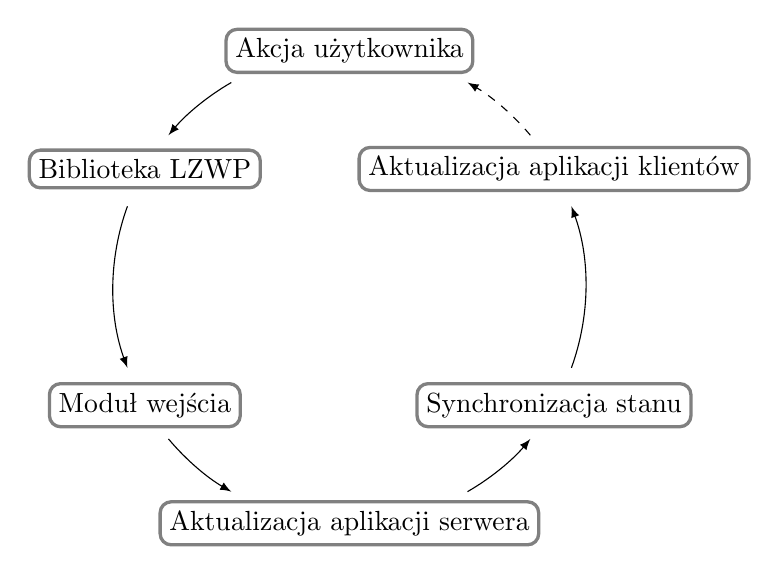
\begin{tikzpicture}[stepstyle/.style={rectangle, 
		rounded corners, draw=gray, very thick,
		text centered, align=center}]
	\def \n {6}
	\def \offset {30}
	\def \radius {3cm}

	\foreach \step [count=\s] in {Akcja użytkownika, Biblioteka LZWP, Moduł wejścia, Aktualizacja aplikacji serwera, Synchronizacja stanu, Aktualizacja aplikacji klientów} {
		\node(\s) [stepstyle] at ({360/\n * (\s) + \offset}:\radius) {\step};
	};
	\foreach \b/\e in {120/140, 160/200, 220/240, 300/320, 340/380} {
		\draw[->, >=latex] ({\b}:\radius)
		arc ({\b}:{\e}:\radius);
	};
		\draw[dashed, ->, >=latex] ({40}:\radius)
		arc ({40}:{60}:\radius);
\end{tikzpicture}
\end{center}
\caption{Diagram kolejności wykonywania modułów przy akcji użytkownika}
\label{fig:diagram-modolow}
\end{figure}



	\section{Zarządzanie pamiecią w aplikacji}
\sectionauthor{Jan Kruczyński}
\label{sec:pamiec}
Ze względu na to, że aplikacja doładowywuje węzły wraz z kolejnymi akcjami użytkownika, gdy przemieszcza się on po grafie lub wskazuje na węzły w przestrzeni, musiał zostać opracowany sposób ich usuwania, by utrzymać płynność działania. Aby to osiągnąć powstał oddzielny kontroler zarządzania pamięcią.

\begin{lstlisting}[caption={Pomocnicze struktury i zmienne kontrolera zarządzania pamięcią}, label=lst:nodePriority]
private List<uint> lowPriorityNodes;%*\label{line:lowPriorityNodes}*)
private List<uint> highPriorityNodes;%*\label{line:highPriorityNodes}*)
public int maxAmountOfNodes;%*\label{line:maxNodes}*)
\end{lstlisting}

Węzły które są załadowane w aplikacji zostały podzielone na dwie kategorie - węzły niskiego priorytetu (\ref{line:lowPriorityNodes}), które są potencjalnymi kandydatami na węzły do usunięcia, oraz wysokiego priorytetu (\ref{line:highPriorityNodes}), których usunąć aktualnie nie można.

Początkowo wszystkie załadowane węzły trafiają do listy niskiego priorytetu. Jeżeli użytkownik dokonuje interakcji z węzłem, to zarówno ten węzeł, jak i wszyscy wyświetlani jego sąsiedzi trafiają do listy wysokiego priorytetu. Jeżeli któryś z tych węzłów znajdował się w liście niskiego priorytetu, jest z niej usuwany i przenoszony na początek listy wysokiego priorytetu.

Funkcjonuje to w taki sposób, aby aplikacja zwalniała w pierwszej kolejności węzły z którymi użytkownik nigdy nie miał interakcji - i dzięki temu nie dostrzegł, że czegoś brakuje. Jednocześnie realizowany jest dodatkowy cel, by ilość wyświetlanych (i przez to przechowywanych w pamięci) węzłów w dowolnej chwili była stała z dokładnością do kilkunastu sztuk.

Kontroler nasłuchuje zdarzenia załadowania węzła przez aplikację. Gdy takie zdarzenie zostanie wykryte, jeżeli liczba wszystkich węzłów, które są wyświetlane w aplikacji, nie przekracza maksymalnej dopuszczonej ilości, nie dzieje się nic. Jeżeli ta liczba zostanie przekroczona, zwalnia kilkanaście węzłów z listy niskiego priorytetu (\ref{line:lowPriorityNodes}).

Gdy lista niskiego priorytetu jest pusta, kontroler przerzuca najstarsze węzły z listy wysokiego priorytetu do listy niskiego priorytetu (są to węzły, z którymi użytkownik prowadził interakcję najdawniej). Gdy użytkownik dokonuje interakcji z węzłem, jest on przerzucany na sam początek listy wysokiego priorytetu.
	\section{Konsola operatora}
\sectionauthor{Mateusz Janicki}
Aplikacja, poza wykorzystaniem flysticków lub klawiatury, może być sterowana za pomocą specjalnej konsoli. Każdorazowe skorzystanie z jaskini wymaga obecności operatora, który uruchamia aplikację w trakcie prezentacji. Będzie on posiadał dostęp do konsoli, a jego zadaniem będzie przenoszenie użytkownika na konkretne węzły przy użyciu wyszukiwarki, a także włączanie zaprogramowanych tras przeglądania grafu. Co więcej, konsola posiada interfejs tworzenia tras umożliwiający szybkie i wygodne tworzenie nowych plików. 

Konsola operatora domyślnie wywoływana jest po naciśnięciu klawisza ''C''. Interfejs posiada dwie zakładki - \textit{Search} oraz \textit{Routes}. Pierwsza jest odpowiedzialna za wyszukiwanie węzłów, na które ma zostać przeniesiony użytkownik, druga służy włączaniu tras. Obydwa elementy posiadają skrypt o nazwie \codeinline{Toggle}, służący odpowiedniemu przełączaniu aktywnych elementów w konsoli. W obu zakładkach znajduje się obiekt przechowujący wyniki wyszukiwania, umieszczane w obiekcie zawierającym komponent  \codeinline{Scroll Rect}. Umożliwia on automatyczne utworzenie paska przewijania, co daje możliwość umieszczenia bardzo dużej ilości elementów.  Dodatkowo w zakładce \textit{Search} znajdują się także obiekt o nazwie  \codeinline{SearchInput} odpowiedzialny za wpisywanie wyszukiwanego węzła, posiadający skrypt  \codeinline{InputField}. Ponadto, nad konsolą znajduje się również informacja o tym, jaki węzeł jest aktualnie wybrany.

\img{\chapterPath/img/console_search.png}{Zrzut ekranu konsoli z otwartą zakładką Search}{console_search}{0.8}
\img{\chapterPath/img/console_routes.png}{Zrzut ekranu konsoli z otwartą zakładką Routes i włączoną trasą}{consoler_routes}{0.8}

Wyszukiwanie węzłów odbywa się na przygotowanym uprzednio pliku, zawierającym posortowane alfabetycznie nazwy artykułów i kategorii oraz ich ID. Przeszukiwanie listy odbywa się za pomocą algorytmu wyszukiwania binarnego. Lista elementów aktualizuje się za każdym wydarzeniem  \codeinline{OnValueChanged} obiektu  \codeinline{SearchInput}. Instancjonowane są kolejne prefaby wyników wyszukiwania, w których zmieniana jest ich pozycja w pionie, nazwa i ikona symbolizująca artykuł lub kategorię. W momencie wybrania węzła wywoływane jest zdarzenie  \codeinline{OnClick}, do którego podpięta jest funkcja  \codeinline{HistoryController} odpowiedzialna za wybranie węzła. Tło wybranego obiektu zmieniane jest na niebiesko.

Lista tras jest pobierana na podstawie aktualnie wybranej wersji Wikipedii. Prefab wyświetlający trasę posiada nazwę, długość trasy oraz przycisk służący jej włączaniu. W celu utworzenia kolejnych elementów listy wykorzystywana jest funkcja  \codeinline{Instantiate()}. W kolejnych instancjach zmieniana jest wysokość obiektu, nazwa przycisku, nazwa trasy oraz długość trasy.  W momencie włączenia trasy wywoływane jest zdarzenie  \codeinline{OnClick}, do którego podpięta jest funkcja  \codeinline{HistoryController} wczytująca trasę o numerze indeksu, którą posiada wciśnięty przycisk. Ponadto tło wybranego obiektu zmieniane jest na niebieski.

	\section{Linia czasu}
\sectionauthor{Mateusz Janicki}
\label{sec:linia-czasu}
Specyfikacja wymagań projektu inżynierskiego zawierała funkcjonalność dotyczącą linii czasu. Wybranie daty miało spowodować wyświetlanie tylko takich węzłów, których data utworzenia była starsza niż wybrana data. Pomogłoby to w przybliżonej wizualizacji, w jak szybki sposób rozrastała się konkretna Wikipedia. Szereg komplikacji spowodował jednak odrzucenie przez nas tej funkcjonalności.

Sterowanie linią czasu miało odbywać się za pomocą drugiego kontrolera. Po wciśnięciu przycisku miał pokazywać się specjalny interfejs ukazujący aktualnie wybraną datę. Można w niej było wybrać, przesuwając joystick w lewo i prawo, miesiąc lub rok, który następnie dałoby się zmieniać przesuwając joystick do góry lub w dół. Zatwierdzenie daty przyciskiem spustu wywoływałoby zmiany w grafie. 

Funkcjonalność nie została zaimplementowana głównie z powodu braku prostej informacji o stworzeniu artykułu w głównie wykorzystywanym przez nas źródle danych, czyli zrzutach baz danych Wikipedii. Istnieją archiwa zawierające kompletną historię edycji artykułów, jednak wielkość tych plików jest nieporównywalnie większa w porównaniu ze zwykłym wykazem stron czy nawet połączeniami pomiędzy stronami. Przetworzenie tych plików tylko po to, aby wydobyć z nich datę pierwszej publikacji strony, jest niewymierna do korzyści wynikających z tej funkcjonalności. 

Innym sposobem wydobycia danych mogłoby być pozyskiwanie tych informacji przy użyciu Wikipedia API. Pomysł ten jednak nie jest wykonalny z powodu ograniczeń, które posiada API. Aby~zdobyć informacje dotyczące każdego artykułu, musielibyśmy wywołać zapytania, których liczba znacznie przewyższa maksymalną dopuszczalną liczbę zapytań dla jednego użytkownika. Przekroczenie tej liczby powoduje zablokowanie adresu IP, z którego pochodziły zapytania i utrudnia dalsze pozyskiwanie danych.

Co więcej, nasza idea linii czasu nie byłaby dokładnym odwzorowaniem stanu Wikipedii w wybranym przez użytkownika czasie. Artykuły i kategorie Wikipedii są bardzo często zmieniane, co implikuje możliwość zmiany połączeń pomiędzy artykułami. Ponadto artykuły i kategorie mogą być także usuwane. Przechowywanie całej historii stron lub stworzenie plików zawierających dokładną historię wszystkich węzłów, jakie kiedykolwiek pojawiły się w Wikipedii, jest niemożliwe na zwykłych komputerach osobistych z powodu zbyt dużej wymaganej przestrzeni na dysku. Nawet jeśli udałoby się je~zapisać, przetwarzanie i wczytywanie takich plików zajęłoby bardzo dużo czasu i spowodowałoby niską responsywność aplikacji. Nasza wersja linii czasu mogłaby być myląca dla nowych użytkowników, którzy mogliby pomyśleć, że przedstawiana jest im dokładna wersja Wikipedii w danym czasie.
	\section{Ostateczny schemat interakcji}
\sectionauthor{Jan Kruczyński}
\label{sec:schemat_interakcji}
Po odrzuceniu funkcjonalności, takich jak widok szczegółowy i linia czasu, możliwa stała się obsługa aplikacji za pomocą tylko jednego kontrolera. Podział na kontroler główny (Rysunek \ref{fig:schemat_kontroler_glowny}) i pomocniczy (Rysunek \ref{fig:schemat_kontroler_pomocniczy}) został odrzucony, a wszystkie interakcje zostały umieszczone na jednym kontrolerze. Ten zabieg znacznie ułatwi użytkownikowi sterowanie aplikacją w jaskini. Nowy schemat sterowania został umieszczony na Rysunku \ref{fig:flystick_new_controls}.

\img{\chapterPath/img/nowy_schemat_kontrolera.png}{Aktualny schemat sterowania kontrolerem}{flystick_new_controls}{0.8}
\end{chapter}



